%!TEX root = ../proteoform_suite_manual.tex
%---------------------------------------------------------------------
%	TOPDOWN
%---------------------------------------------------------------------

\section{Top-Down}

\subsection{Overview}
On this page, the top-down hit results are read in from the file(s) loaded under Top-Down Hit Results on the Load Results page. A top-down hit is a proteoform spectral match. Top-down hits are then aggregated into top-down  proteoforms by identification and retention time. The theoretical database is supplemented with top-down proteoform identifications not already present in the database. Bottom-up peptide results are integrated with the top-down proteoform results.

\subsection{Run Page}
\begin{itemize}
\item Load top-down results file(s) on the Load Results page under Top-Down Hit Results (see \textbf{Load Results} section)
\item Set all parameters as desired for current analysis (see below)
\item Click Run Page button (top right)
\end{itemize}

\subsection{Set Parameters}
\begin{figure}[h]
\centering
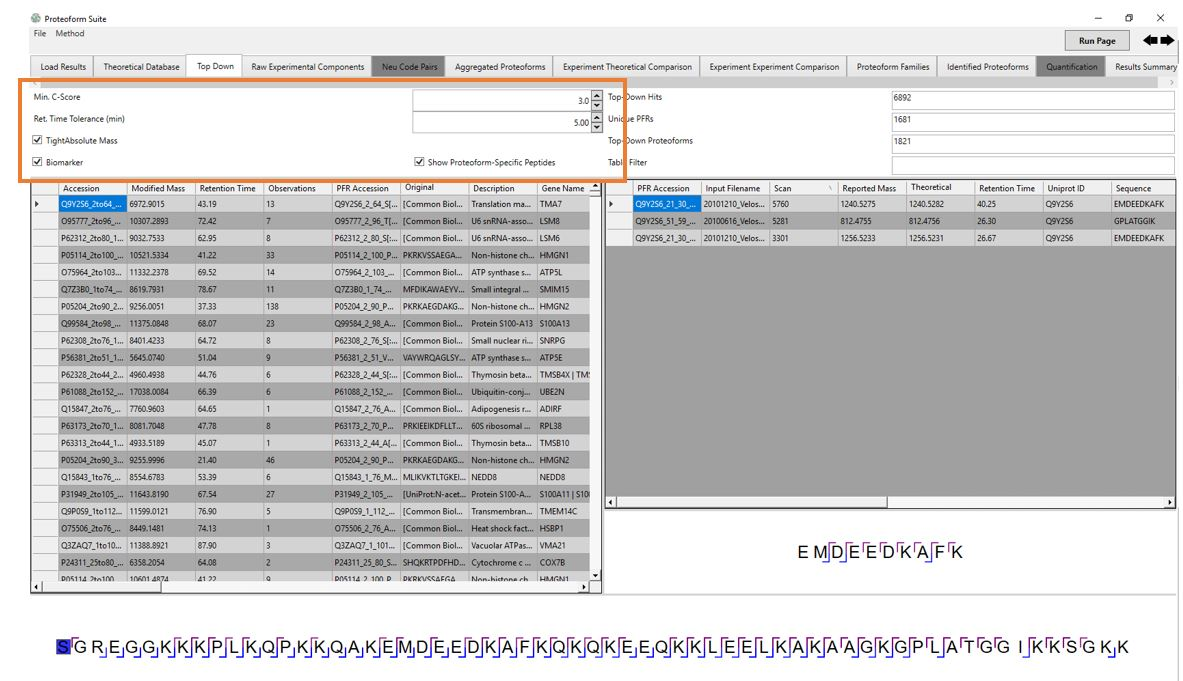
\includegraphics[scale=0.42]{figures/topdown1.jpg}
\end{figure}
\begin{itemize}
\item Min. C-Score: the minimum C-score\supercite{LeDuc2014} for TDPortal results required for a top-down hit to be included. C-scores of 3 and higher correspond to identified proteoforms and C-scores of 40 and higher correspond to well-characterized proteoforms
\item Ret. Time Tolerance (min): retention time tolerance used for aggregated top-down hits of the same proteoform identifications. Top-down hits of the same ID that elute outside of this tolerance will be aggregated into separate top-down proteoforms
\item Tight Absolute Mass: if checked, TDPortal hits from the Tight Absolute Mass search will be included
\item Biomarker: if checked, TDPortal hits from the Biomarker search will be included
\end{itemize}

\subsection{Results}
\begin{itemize}
	\item Top-Down Hits: total number of top-down hits (proteoform spectral matches)
	\item Unique PFRs: unique proteoform identifications
	\item Top-Down Proteoforms: number of aggregated top-down proteoforms. May be greater than the number of unique PFRs if some hits of the same ID fall outside of the retention time tolerance
	\item Table Filter: filter the Top-Down Proteoforms table (left) by any entered text
		\begin{figure}[h]
\centering
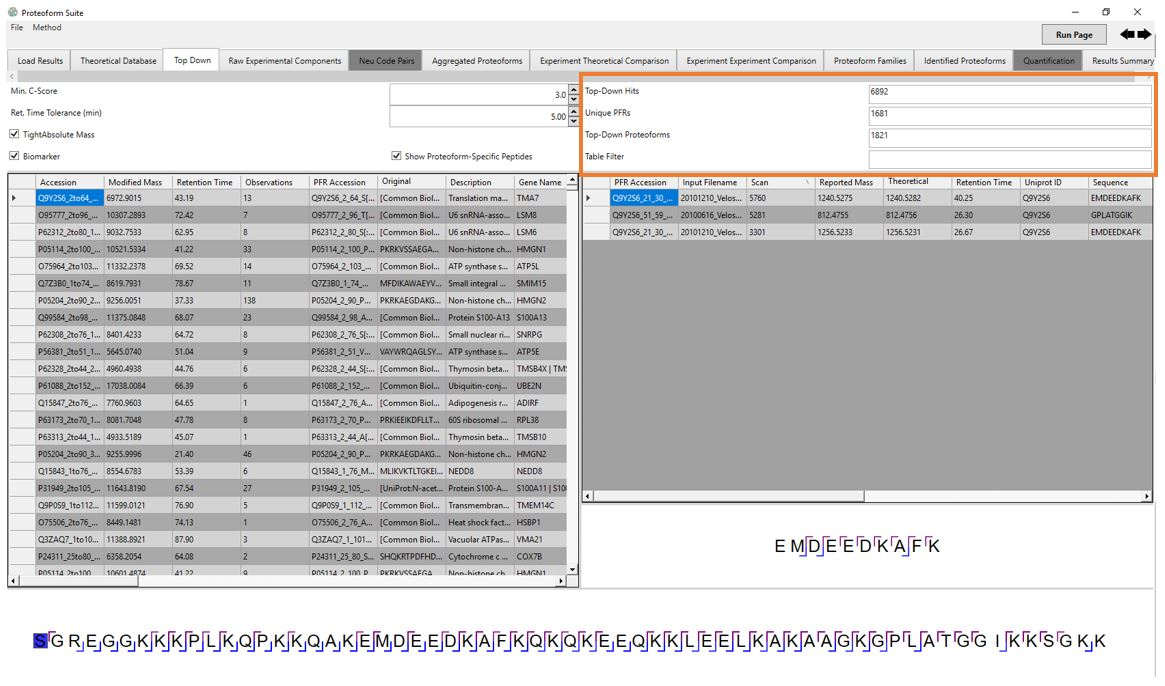
\includegraphics[scale=0.42]{figures/topdown2.jpg}
\end{figure}
	\newpage
	\item Top-down Proteoforms table: the left table displays all top-down proteoforms. For MetaMorpheus results, ambiguous identifications in a single top-down proteoform have information separated by a "|". 
	\begin{figure}[h]
\centering
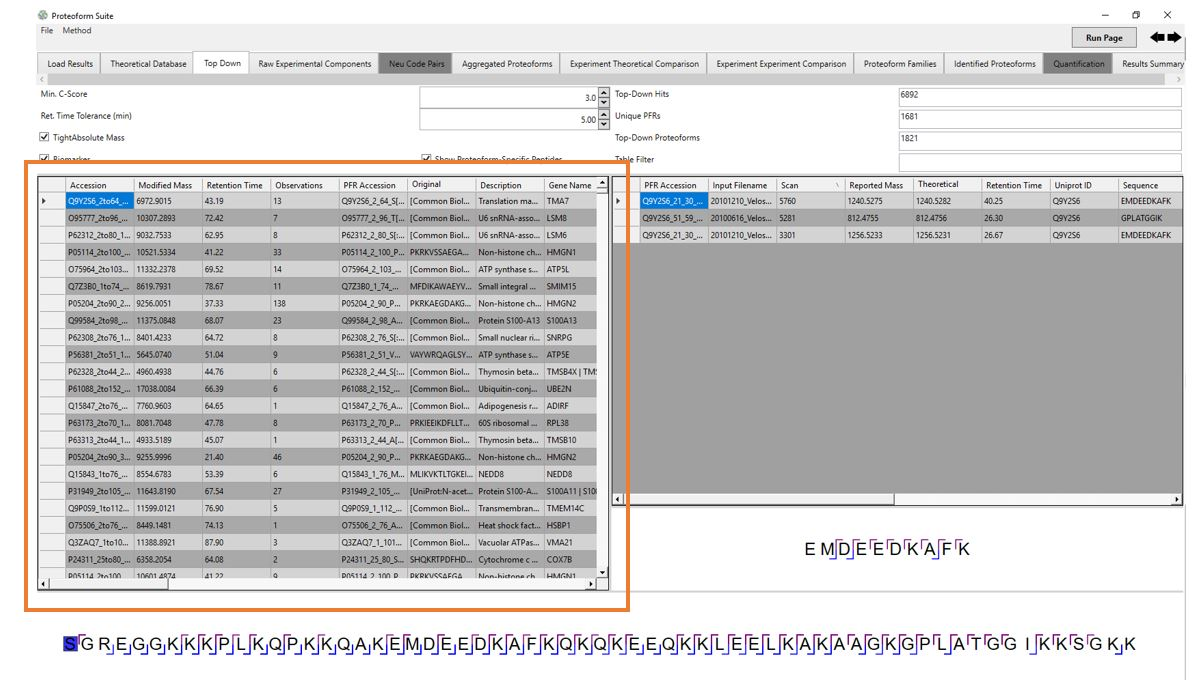
\includegraphics[scale=0.42]{figures/topdown3.jpg}
\end{figure}
	\begin{itemize}
		\item Accession: accession given by Proteoform Suite for this specific top-down proteoform
		\item Modified Mass: monoisotopic mass of top-down proteoform (average of aggregated top-down hits)
		\item Retention Time: retention time of top-down proteoform (average of aggregated top-down hits)
		\item Observations: number of aggregated top-down hits in this top-down proteoform
		\item PFR Accession: protein accession\_begin residue\_end residue\_full sequence with PTMs
		\item Original PFR Accession/full-sequence: PFR accession in TDPortal, full sequence reported in MetaMorpheus
		\item Description: protein description from UniProt
		\item Gene Name: gene name from UniProt
		\item UniProt ID: protein UniProt ID
		\item Accessions: UniProt protein accession
		\item PTM Description: PTMs on top-down proteoform
		\item Begin and End: top-down proteoform begin and end residue in protein full sequence in UniProt
		\item Sequence: top-down proteoform sequence
		\item UniProt-Annotated Modifications: all UniProt annotated residues for PTMs on this top-down proteoform in UniProt database provided
		\item Potentially Novel Mods: checked if this top-down proteoform contains PTMs not annotated in UniProt database provided
		\item Best Hit Score: best C-score (TDPortal) or MetaMorpheus score (MetaMorpheus) out of aggregated hits for this top-down proteoform
		\item Best Hit Delta Score: best delta score (score difference between next best scoring identification) out of aggregated hits for this top-down proteoform (MetaMorpheus results only)
		\item Best Hit Q-Value: best q-value out of aggregated hits for this top-down proteoform
		\item Level: proteoform identification level based on five-level scheme\supercite{Smith2019b}
		\item Level Description: description of proteoform level assignment (sources of ambiguity)
		\item Mass Error: difference in mass between experimental and theoretical proteoform monoisotopic mass
		\item Best Hit Info: filename for highest scoring hit aggregated into this top-down proteoform
		\item Family: proteoform family number (must have run through full Proteoform Suite analysis)
		\item Linked Proteoform References: proteoforms in family network path of identification to the nearest theoretical proteoform (must have run through full Proteoform Suite analysis)
		\item Bottom-Up PSMs Count: number of bottom-up PSMs derived from this top-down proteoform
		\item Different Ambiguity in Bottom-Up PSMs: checked for ambiguous top-down identifications where the different IDs have a different number of bottom-up PSMs
		\item Modified Bottom-Up PSMs: modified residues confirmed by ID'd bottom-up peptides derived from this top-down proteoform
		\item All Modified Bottom-Up PSMs from Protein: modified residues confirmed by ID'd bottom-up peptides derived from this top-down proteoform's protein
		\item Bottom-Up PSMs Separate Peptides: modified residues confirmed ID'd by bottom-up peptides derived from this top-down proteoform, keeping unique peptidoforms separate
		\item Bottom-Up Evidence for Begin: checked if bottom-up peptide identified with begin residue at this top-down proteoform's begin residue
		\item Bottom-Up Evidence for End: checked if bottom-up peptide identified with end residue at this top-down proteoform's end residue
		\item Bottom-Up Evidence for All PTMs: checked if all PTMs on this top-down proteoform are confirmed by at least one modified bottom-up peptide
		\item Sequence Specific: description of difference in PTMs between bottom-up peptides from this top-down proteoform sequence and this top-down proteoform's PTMs
		\item All Peptides from Protein: description of difference in PTMs between bottom-up peptides from this top-down proteoform's protein and this top-down proteoform's PTMs
		\item Fragments: if MetaMorpheus results, MS/MS fragments identified
	\end{itemize}
		\begin{figure}[h]
\centering
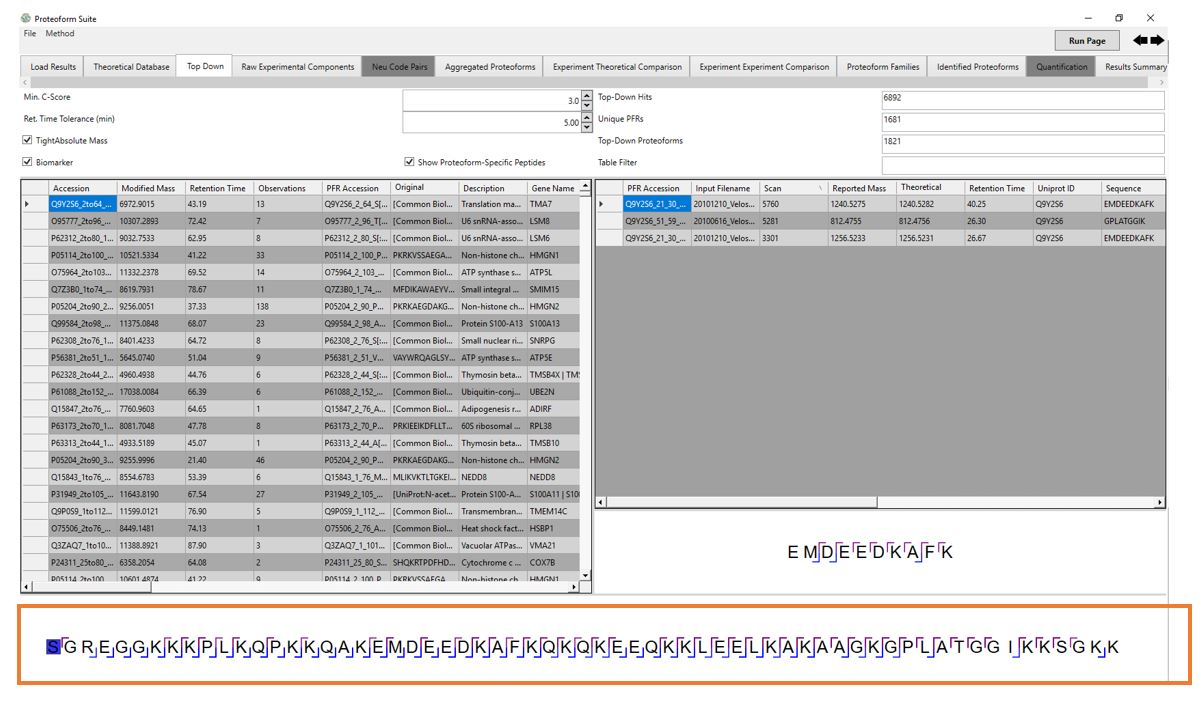
\includegraphics[scale=0.42]{figures/topdown4.jpg}
\end{figure}
	\item Top-down Proteoform Sequence box: bottom box on page where sequence is displayed with PTMs for the top-down proteoform selected in the Top-Down Proteoforms table (left). If MetaMorpheus results, sequence is annotated based on identified MS/MS fragments
	\item Show Proteoform-Specific Peptides: if checked, only peptides specific to the selected top-down proteoform in the Top-Down Proteoform table (left) are displayed in the Bottom-Up Peptide table (right). If unchecked, all bottom-up peptides from the top-down proteoform's protein are displayed. 
	\item Bottom-Up Peptides table: the right table displays bottom-up peptides from the top-down proteoform selected in the Top-Down Proteoforms table (left) if Show Proteoform-Specific Peptides is checked. The right table displays all bottom-up peptides from the top-down proteoform's protein selected in the Top-Down Proteoforms table (left) if Show Proteoform-Specific Peptides is unchecked. 
	\begin{figure}[h]
\centering
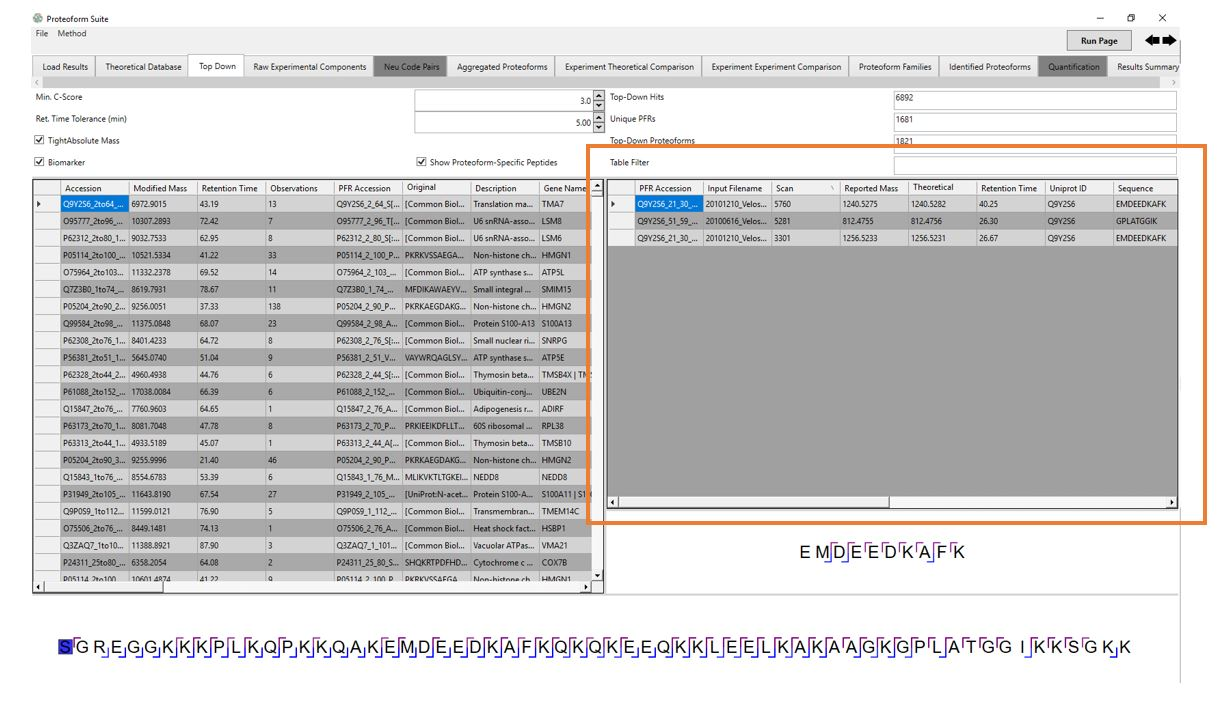
\includegraphics[scale=0.42]{figures/topdown5.jpg}
\end{figure}
	\begin{itemize}
		\item PFR Accession: protein accession\_begin residue\_end residue\_full sequence with PTMs
		\item Input Filename: filename for this bottom-up peptide identification
		\item Scan: scan number for this bottom-up peptide identification
		\item Reported Mass: observed monoisotopic mass for this bottom-up peptide identification
		\item Theoretical Mass: theoretical mass for this bottom-up peptide identification
		\item Retention Time: retention time for this bottom-up peptide identification
		\item UniProt ID: protein UniProt ID
		\item Sequence: peptide sequence
		\item Begin: peptide begin residue in protein full sequence in UniProt
		\item End: peptide end residue in protein full sequence in UniProt
		\item PTM Description: PTMs on peptide
		\item Accession: UniProt protein accession
		\item Name: name of protein from UniProt
		\item Q-value: PEP q-value for this bottom-up peptide
		\item Score: MetaMorpheus score for this peptide
		\item Shared: checked if this peptide is a shared peptide between multiple proteins
	\end{itemize}
	\item Bottom-Up Sequence box: middle right box on page where sequence is displayed with PTMs for the peptide selected in the Bottom-Up Peptides table (right). If MetaMorpheus results, sequence is annotated based on identified MS/MS fragments
	\begin{figure}[h]
\centering
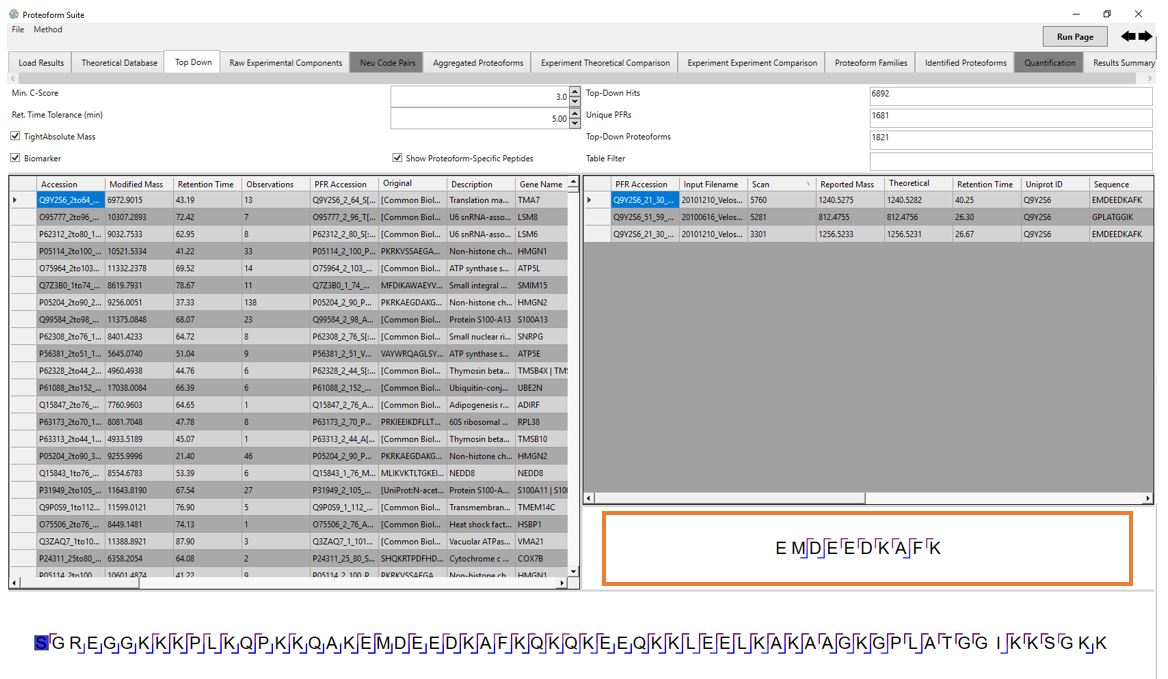
\includegraphics[scale=0.42]{figures/topdown6.jpg}
\end{figure}
\end{itemize}